\documentclass[crop,tikz]{standalone}
\usetikzlibrary{backgrounds}
\colorlet{blue}{cyan}
\tikzset{
  inverted/.style = {
    color=white,
    background rectangle/.style={fill},
    show background rectangle
  }
}

\usepackage{pgfplots}
\tikzset{>=latex}

\begin{document}
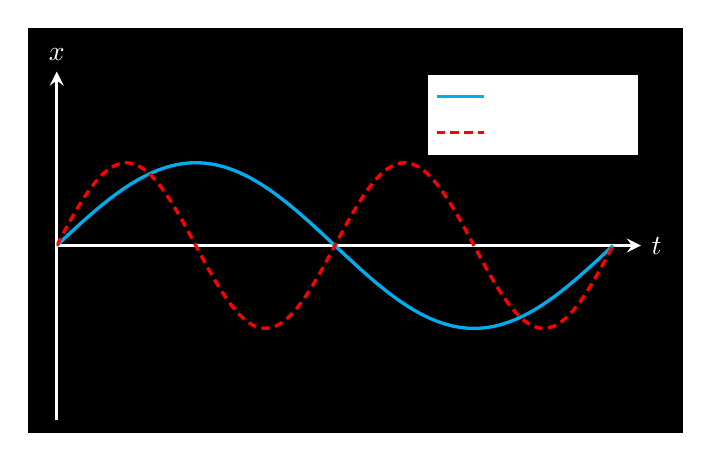
\begin{tikzpicture}[inverted,inverted]
\begin{axis}[
  very thick,
  width=9cm,
  height=6cm,
  domain={0}:{2*pi},
  samples=50,
  axis y line=middle,
  axis x line=middle,
  xlabel={$t$},
  ylabel={$x$},
  xlabel style={right},
  ylabel style={above},
  xmin=0, xmax={2.1*pi},
  ymin=-2.1, ymax=2.1,
  xtick={\empty},
  xticklabels={\empty},
  ytick={\empty},
  yticklabels={\empty},
  legend cell align={left},
  legend style={at={(1,1)},anchor=north east}
  ]
  \addplot[blue,smooth] { sin(deg(x)) };
  \addlegendentry{$A\sin(\omega_0 t)$};
  \addplot[red,smooth,densely dashed] { sin(deg(2*x)) };
  \addlegendentry{$A\sin(2\omega_0 t)$};
\end{axis}
\end{tikzpicture}
\end{document}
